\documentclass[11pt,a4paper]{article}
\usepackage[utf8]{inputenc}
\usepackage[french]{babel}
\usepackage{amsmath}
\usepackage{amsfonts}
\usepackage{pifont} 
\usepackage{amssymb}
\usepackage{calc}
\usepackage{makeidx}
\usepackage{multicol}
\usepackage{graphicx} 
\usepackage{shadow}
\usepackage{algorithm}
\usepackage{eurosym}
\usepackage{pst-all} 
\usepackage{pst-plot} 
\usepackage{lastpage}
\usepackage{pstricks-add}
\usepackage{pstricks,pst-plot,pst-text,pst-tree,pst-eps,pst-fill,pst-node,pst-math,pst-blur,pst-func}
\usepackage{logsys}
\usepackage{pythontex}
\def \Oij{$(O;\overrightarrow{i};\overrightarrow{j})$}
\newcommand{\vect}[1]{$\overrightarrow{#1}$}
\usepackage{tabvar} 
\usepackage{cancel}
\usepackage{ifthen,ifpdf,etoolbox,xkeyval}
\usepackage{tcolorbox}
\tcbuselibrary{skins}
\usepackage{tikz,tikzsymbols,tkz-tab}
\usepackage{vmargin}
\setmarginsrb{1cm} {0.5cm}{1cm}{1cm}{1cm}{0.5cm}{1cm}{1cm}
\renewcommand{\thefootnote}{%
\ding{45}}
\usepackage{mdframed}
\usepackage{ifthen}
\usepackage{ifpdf}
\usepackage{etoolbox}
\usepackage{listings}
\usepackage{sectsty}
\usepackage{pifont}
\frenchbsetup{StandardLists=true} % à inclure si on utilise \usepackage[french]{babel}
\usepackage{enumitem}
%%%%%%%%%%%%%%%%%%%%%%%%%%%%%%%%%%%%%%%%%%%%%%%%%%%%%%%%%%%%%%%%%%%%%%%%%%%%%%%%%%
%%%%%%%%%%%%%%%MARGE%%%%%%%%%%%%%%%%%%%%%%%%%%%%%%%%%%%%%%%%%%%%%%%%%
\usepackage{vmargin}
\setmarginsrb{1cm} {0cm}{1cm}{1cm}{1cm}{0.5cm}{1cm}{1cm}
%%%%%%%%%%%%%%%%%%%%%%%%%%%%%%%%%%%%%%%%%%%%%%%%%%%%%%%%%%%%%%%%%%%%%%%%%%%%
\usepackage{sectsty}
\sectionfont{\color{red}{}}
\subsectionfont{\color{blue}{}}
\usepackage{titlesec}
%Voir p156 pour les paramètres
\titleformat{\section}[frame]%
{\titleline[r]{}\normalfont}%
{\filcenter%
\texttt{~Section \thesection~}}%
{5pt}{\Large \bfseries\filcenter}{}
%%%%%%%%%%%%%%%%%%%%%%%%%%%%%%%%%%%%%%%%%%%%%%%%%%%%%%%%%%%%%%%%%%%%%%%%%%%%%%%%%%
%%%%%%%%%%%%%%%%%%%%%%%%%%%%%%%%%%%%%%%%%%%%%%%%%%%%%%%%%%%%%%%%%%%%%%%%%%%%%%%%%%

%%%%%%%%%%%%%%%%%%%%%%%%%%%%%%%%%%%%%%%%%%%%%%%%%%%%%%%%%%%%%%%%%%%%%%%%%%%%%%%%%%
%%%%%%%%%%%%%%%%%%%%%%%%%%%%%%%%%%%%%%%%%%%%%%%%%%%%%%%%%%%%%%%%%%%%%%%%%%%%%%%%%%

%%%%%%%%%%%%%%%%%%%%%%%%%%%%%%%%%%%%%%%%%%%%%%%%%%%%%%%%%%%%%%%%%%%%%%%%%%%%%%%%%%
%%%%%%%%%%%%%%%%%%%%%%%%%%%%%%%%%%%%%%%%%%%%%%%%%%%%%%%%%%%%%%%%%%%%%%%%%%%%%%%%%%
\renewcommand{\thefootnote}{%
\ding{45}}
%%%%%%%%%%%%%%%%%%%%%%%%%%%%%%%%%%%%%%%%%%%%%%%%%%%%%%%%%%%%%%%%%%%%%%%%%%%%%%%%%%
%%%%%%%%%%%%%%%%%%%%%%%%CODE POUR PYTHON%%%%%%%%%%%%%%%%%%%%%%%%%%%%%%%%%%%%%%%%%%
%%%%%%%%%%%%%%%%%%%%%%%%%%%%%%%%%%%%%%%%%%%%%%%%%%%%%%%%%%%%%%%%%%%%%%%%%%%%%%%%%%
%%%%%%%%%%%%%%%%%%%%%%%%%%%%%%%%%%%%%%%%%%%%%%%%%%%%%%%%%%%%%%%%%%%%%%%%%%%%%%%%%%
%%%%%%%%%%%%%%%%%%%%%%%%CODE POUR EXO%%%%%%%%%%%%%%%%%%%%%%%%%%%%%%%%%%%%%%%%%%
%%%%%%%%%%%%%%%%%%%%%%%%%%%%%%%%%%%%%%%%%%%%%%%%%%%%%%%%%%%%%%%%
\definecolor{mygreen}{rgb}{0.1,0.8,0.1}
\definecolor{mygray}{rgb}{0.5,0.5,0.5}
\definecolor{souris}{gray}{0.85}
\definecolor{mymauve}{rgb}{0.58,0,0.82}
\definecolor{darkWhite}{rgb}{0.94,0.94,0.94}
\lstset{
  aboveskip=3mm,
  belowskip=-2mm,
  backgroundcolor=\color{darkWhite},
  basicstyle=\footnotesize,
  breakatwhitespace=false,
  breaklines=true,
  captionpos=b,
  commentstyle=\color{red},
  deletekeywords={...},
  escapeinside={\%*}{*)},
  extendedchars=true,
  framexleftmargin=16pt,
  framextopmargin=3pt,
  framexbottommargin=6pt,
  frame=tb,
  keepspaces=true,
  keywordstyle=\color{blue},
  language=Python,
  literate=
  {²}{{\textsuperscript{2}}}1
  {⁴}{{\textsuperscript{4}}}1
  {⁶}{{\textsuperscript{6}}}1
  {⁸}{{\textsuperscript{8}}}1
  {€}{{\euro{}}}1
  {é}{{\'e}}1
  {è}{{\`{e}}}1
  {ê}{{\^{e}}}1
  {ë}{{\¨{e}}}1
  {É}{{\'{E}}}1
  {Ê}{{\^{E}}}1
  {û}{{\^{u}}}1
  {ù}{{\`{u}}}1
  {â}{{\^{a}}}1
  {à}{{\`{a}}}1
  {á}{{\'{a}}}1
  {ã}{{\~{a}}}1
  {Á}{{\'{A}}}1
  {Â}{{\^{A}}}1
  {Ã}{{\~{A}}}1
  {ç}{{\c{c}}}1
  {Ç}{{\c{C}}}1
  {õ}{{\~{o}}}1
  {ó}{{\'{o}}}1
  {ô}{{\^{o}}}1
  {Õ}{{\~{O}}}1
  {Ó}{{\'{O}}}1
  {Ô}{{\^{O}}}1
  {î}{{\^{i}}}1
  {Î}{{\^{I}}}1
  {í}{{\'{i}}}1
  {Í}{{\~{Í}}}1,
  morekeywords={*,...},
  numbers=left,
  numbersep=10pt,
  numberstyle=\tiny\color{black},
  rulecolor=\color{black},
  showspaces=false,
  showstringspaces=false,
  showtabs=false,
  stepnumber=1,
  stringstyle=\color{gray},
  tabsize=4,
  title=\lstname,
}
%%%%%%%%%%%%%%%%%%%%%%%%%%%%%%%%%%%%%%%%%%%%%%%%%%%%%%%%%%%%%%%%
\newcounter{exo} 
\setcounter{exo}{0}
\newcommand{\exo}[2][]%
{ 
\addtocounter{exo}{1}
\begin{tcolorbox}[enhanced, arc=1ex,left=3pt,right=3pt,top=3pt,colframe=blue!50!black,colback=white, title = Exercice \theexo~#1\black, attach boxed title to top left=
{xshift=-2mm,yshift=-2mm},
boxed title style={size=small,colback=blue},]
#2
\end{tcolorbox}

}
%%%%%%%%%%%%%%%%%%%%%%%%%%%%%%%%%%%%%%%%%%%%%%%%%%%%%%%%%%%%%%%%
\newcounter{ques} 
\setcounter{ques}{0}
\newcommand{\qst}[2][]%
{ 
\addtocounter{ques}{1}
\hrule
%vspace{0.1cm}
\textbf{Question\theques~#1\black }
#2
\vspace{0.25cm}
\hrule
}
%%%%%%%%%%%%%%%%%%%%%%%%%%%%%%%%%%%%%%%%%%%%%%%%%%%%%%%%%%%%%%%%
\newcounter{exem} 
\setcounter{exem}{0}
\newcommand{\exemcrs}[2][]%
{ 
\addtocounter{exem}{1}
\begin{tcolorbox}[enhanced, arc=1ex,left=3pt,right=3pt,top=3pt,colframe=blue!50!black,colback=white, title = Exemple \theexem~#1\black, attach boxed title to top center]
#2
\end{tcolorbox}
}
%%%%%%%%%%%%%%%%%%%%%%%%%%%%%%%%%%%%%%%%%%%%%%%%%%%%%%%%%%
\newcounter{def} 
\setcounter{def}{0}
\newcommand{\defcrs}[2][]%
{ 
\addtocounter{def}{1}
\begin{tcolorbox}[enhanced, arc=1ex,left=3pt,right=3pt,top=3pt,colbacktitle=white,colback=blue!10!white,coltitle=red!70!black, title = Définition \thedef~#1\black, fonttitle=\sffamily\bfseries\large ]
#2
\end{tcolorbox}
}
%%%%%%%%%%%%%%%%%%%%%%%%%%%%%%%%%%%%%%%%%%%%%%%%%%%%%%%%%%%%%%
%%%%%%%%%%%%%%%%%%%%%%%%%%%%%%%%%%%%%%%%%%%%%%%%%%%%%%%%%%
\newcounter{prop} 
\setcounter{prop}{0}
\newcommand{\defprop}[2][]%
{ 
\addtocounter{prop}{1}
\begin{tcolorbox}[enhanced, arc=1ex,left=3pt,right=3pt,top=3pt,colbacktitle=white,colback=blue!10!white,coltitle=red!70!black, title =Propriété \theprop~#1\black, fonttitle=\sffamily\bfseries\large ]
#2
\end{tcolorbox}
}
%%%%%%%%%%%%%%%%%%%%%%%%%%%%%%%%%%%%%%%%%%%%%%%%%%%%%%%%%%
%%%%%%%%%%%%%%%%%%%%%%%%%%%%%%%%%%%%%%%%%%%%%%%%%%%%%%%%%%%%%%
%%%%%%%%%%%%%%%%%%%%%%%%%%%%%%%%%%%%%%%%%%%%%%%%%%%%%%%%%%%%%%%%%%%%%%%%%%%%%%%%%%
%%%%%%%%%%%%%%%%%%%%%%%%CODE POUR IDEE%%%%%%%%%%%%%%%%%%%%%%%%%%%%%%%%%%%%%%%%%%
%%%%%%%%%%%%%%%%%%%%%%%%%%%%%%%%%%%%%%%%%%%%%%%%%%%%%%%%%%%%%%%%%%%%%%%%%%%%%%%%%%
%%%%%%%%%%%%%%%%%%%%%%%%%%%%%%%%%%%%%%%%%%%%%%%%%%%%%%%%%%%%%%%%%%%%%%%%%%%%%%%%%%
\usepackage{fancyhdr}
\pagestyle{fancy}
\renewcommand{\headrulewidth}{0.5pt}
\renewcommand{\footrulewidth}{0.5pt}
\fancyhead[L]{Signaux analogiques et numériques}
\fancyhead[R]{BTS SN}
\fancyfoot[R]{\textbf{page \thepage}} 
\fancyfoot[L]{Lycée de Baudre}
%\fancyfoot[C]{BTS SN}
%%%%%%%%%%%%%%%%%%%%%%%%%%%%%%%%%%%%%%%%%%%%%%%%%%%%%%%%%%%%%%%%%%%%%%%%%%%%%%%%%%
%%%%%%%%%%%%%%%PRESENTATION DOC%%%%%%%%%%%%%%%%%%%%%%%%%%%%%%%%%%%%%%%%%%
\newcommand{\doc}[1]{\fbox{
\begin{minipage}{0.95\linewidth}
 \classedoc  \hfill BTS SN \\
\vspace{0.1cm}
\begin{center}\begin{LARGE}
\textbf{TP:#1 }\end{LARGE} \end{center}
\vspace{0.1cm}
\end{minipage}}\vspace{0.2cm}%
}
%%%%%%%%%%%%%%%%%%%%%%%%%%%PARAMETRE%%%%%%%%%%%%%%%%%%%%%%%%%%%%%%%%
\def\classedoc{\begin{Large}Fiche informatique \end{Large}}
%%%%%%%%%%%%%%%%%%%%%%%%%%%P%%%%%%%%%%%%%%%%%%%%%%%%%%%%%%%%
\usepackage{tikz}
\usetikzlibrary{babel}
\usepackage[european]{circuitikz}

%%%%%%%%%%%%%%%%%%%%%%%%%%%%%%%%%%%%%%%%%%%%%%%%%%%%%%%
%\author{Marc TURRO}

\title{\textbf{Un peu de théorie sur les signaux...}}
\date{}
%\hline

\begin{document}
\maketitle
\tableofcontents
\newpage
\section{Le problème!}
Lorsque un guitariste pince la corde de \texttt{La}(deuxième en partant du haut) à vide, un son se produit. C'est une perturbation physique de l'environnement qui permet son transfert jusqu'à nos oreilles. On peut représenter l'évolution de ce signal de deux façons:
\begin{itemize}[label = \ding{235}]
\item Une représentation \textbf{temporelle} qui montre comment évolue l'amplitude du son en fonction du \textbf{temps}:\\
\begin{minipage}{0.5\linewidth}
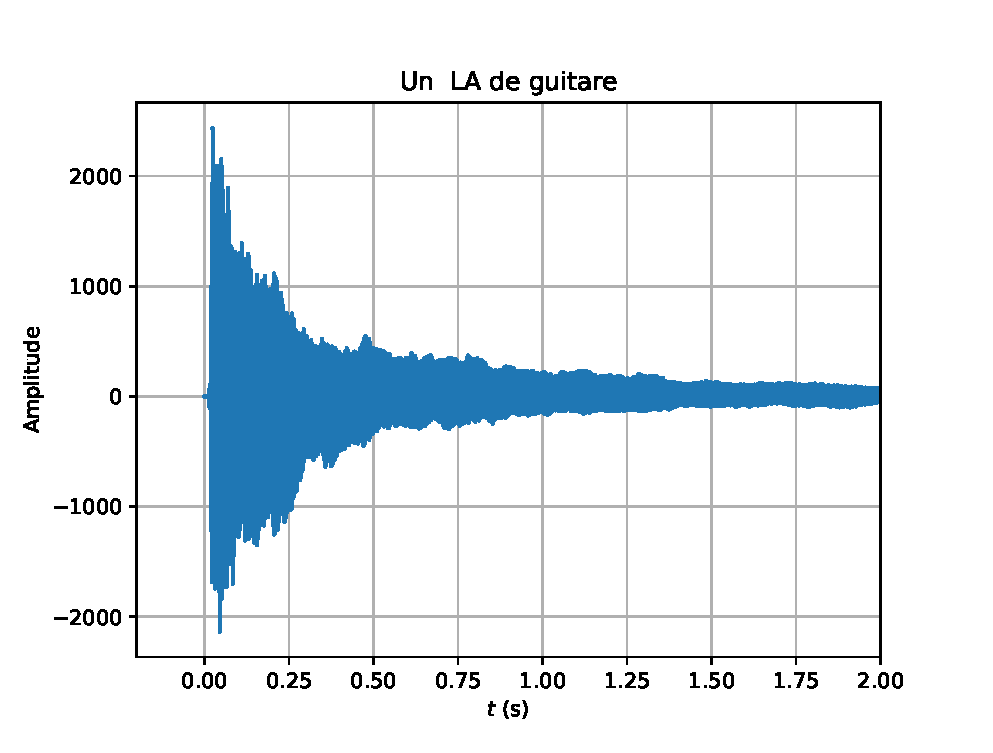
\includegraphics[scale=0.5]{la_guitare.eps} 

\end{minipage}
\begin{minipage}{0.5\linewidth}
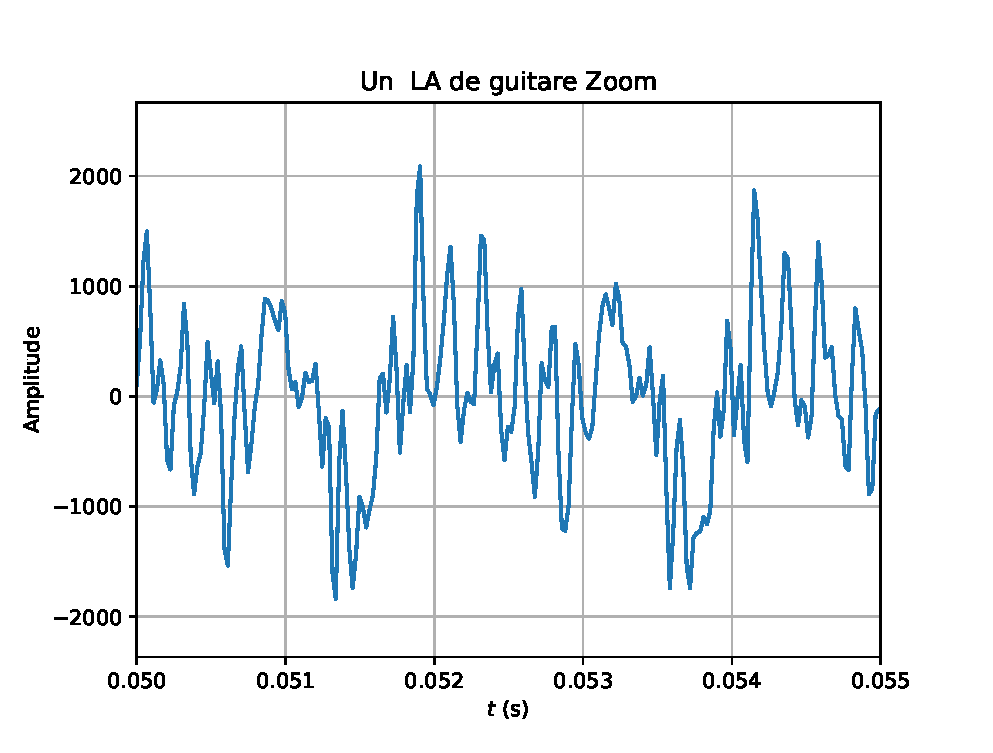
\includegraphics[scale=0.5]{la_guitare_zoom.eps} 

\end{minipage}
\item Une représentation \textbf{fréquentielle} qui montre comment évolue l'amplitude du son en fonction des \textbf{fréquences} qu'il contient:\\
\begin{center}
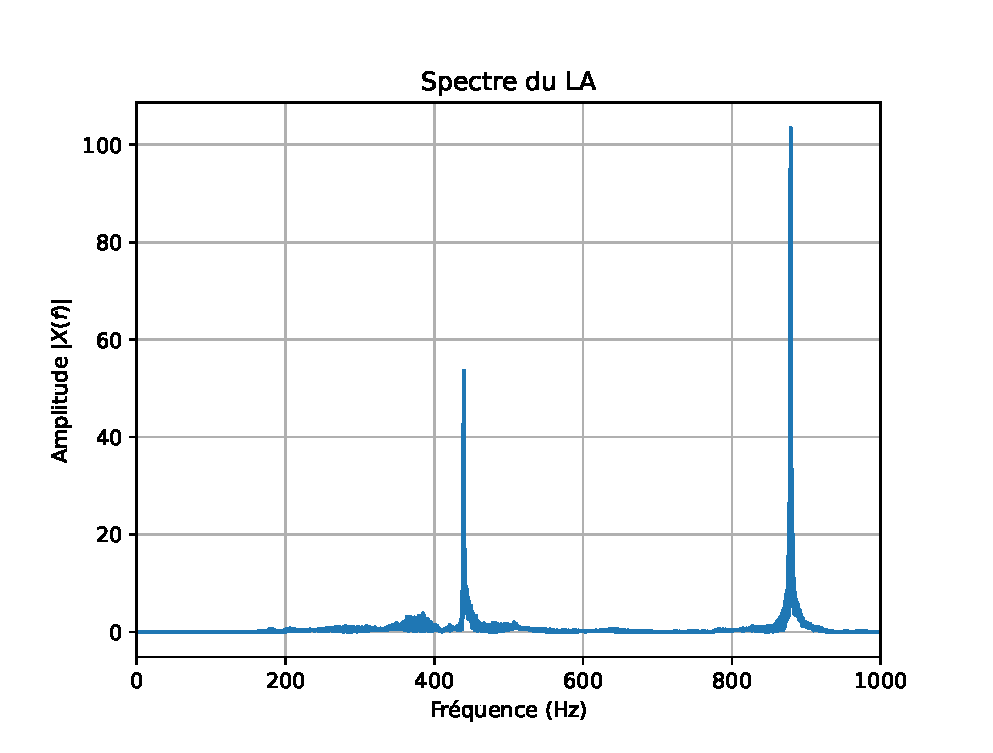
\includegraphics[scale=0.5]{spectre_la.eps} 
\end{center}
\end{itemize}
Le spectre permet de connaître le contenu fréquentiel d'un signal: la fondamentale du LA guitare cinquième corde, est $440Hz$ et la première harmonique à $880Hz$.\\
Lorsqu'on transmet un signal, audio par exemple, plusieurs questions s'offrent à nous:\\
\begin{itemize}[label = \ding{235}]
\item  le signal est-il bien livré?
\item sa composition spectrale est-elle conservée?

\end{itemize}
Nous répondrons en partie à ces questions, en particulier lorsqu'il s'agit de signaux numérisés, qui par nature sont déjà détériorés!

\newpage
\section{Types de signaux}
Il existe de nombreux types de signaux:\\
\begin{itemize}[label = \ding{235}]
\item \textbf{déterministes}, qui peuvent être définis préalablement, en particulier par une fonction mathématique; 
\item \textbf{aléatoires}, dont le comportement ne dépend de paramètres extérieurs.

\end{itemize}
On appelle \textbf{bruit}, tout signal ajouter à un signal déterministe qui peut donc en modifier la nature. Le bruit est en général, un signal aléatoire.\\
On distinguera aussi les signaux \textbf{analogiques} des signaux \textbf{numériques}, obtenus à partir des premiers, par une chaîne de numérisation dont nous rappellerons le principe un peu plus loin plus tard dans ce cours...\\
Un signal analogique est un signal continue au sens mathématiques du terme, alors qu'un signal numérisé est un signal discret (toujours au sens mathématique du terme): il n'existe que pour certaines valeurs de la variable temps $t$.\\
\begin{center}
\begin{minipage}{0.45\linewidth}
\includegraphics[scale=0.5]{sin_num1.eps} 

\end{minipage}\hfill
\begin{minipage}{0.45\linewidth}
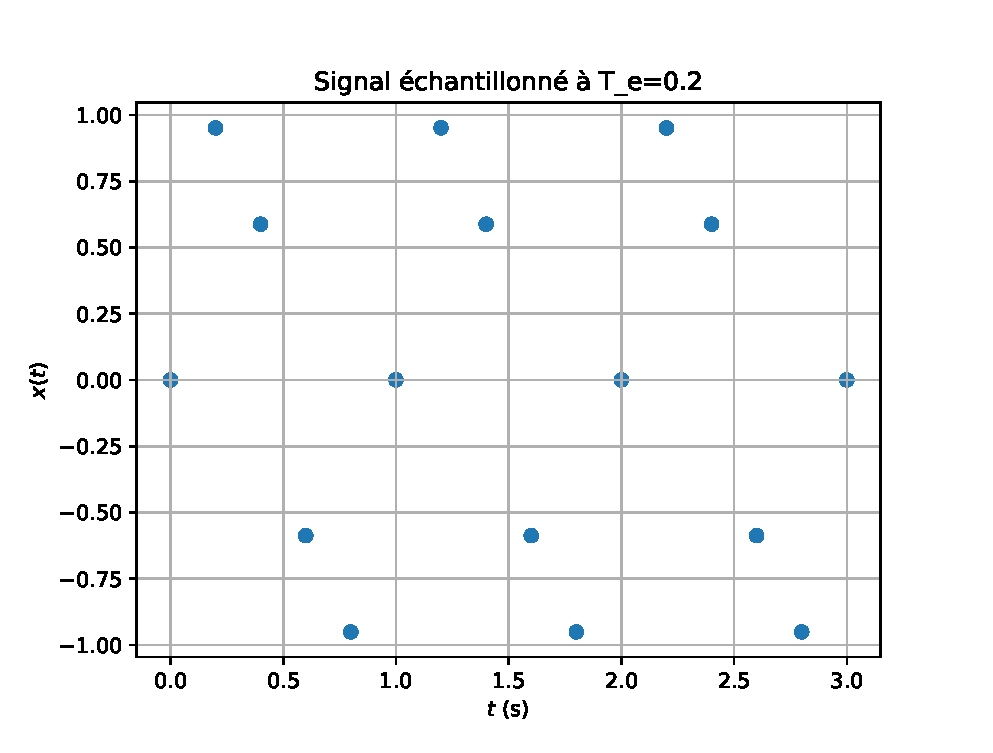
\includegraphics[scale=0.5]{sin_num2.eps} 

\end{minipage}
\end{center}
Le signal numérique n'existe qu'au instant $t=k\times T_e$ où $k$ est un entier ($k\in \mathbb{N}$)et $T_e$ la période d'échantillonnage.


\section{Analyse de Fourier}
Il existe des situations où il est très simple de déterminer le spectre d'un signal. Quant un signal peut être modélisé par une fonction sinusoïdale, la construction du spectre est immédiate:\\
\begin{minipage}{0.5\linewidth}
\includegraphics[scale=0.5]{sinus_4pi.eps} 

\end{minipage}\hfill
\begin{minipage}{0.5\linewidth}
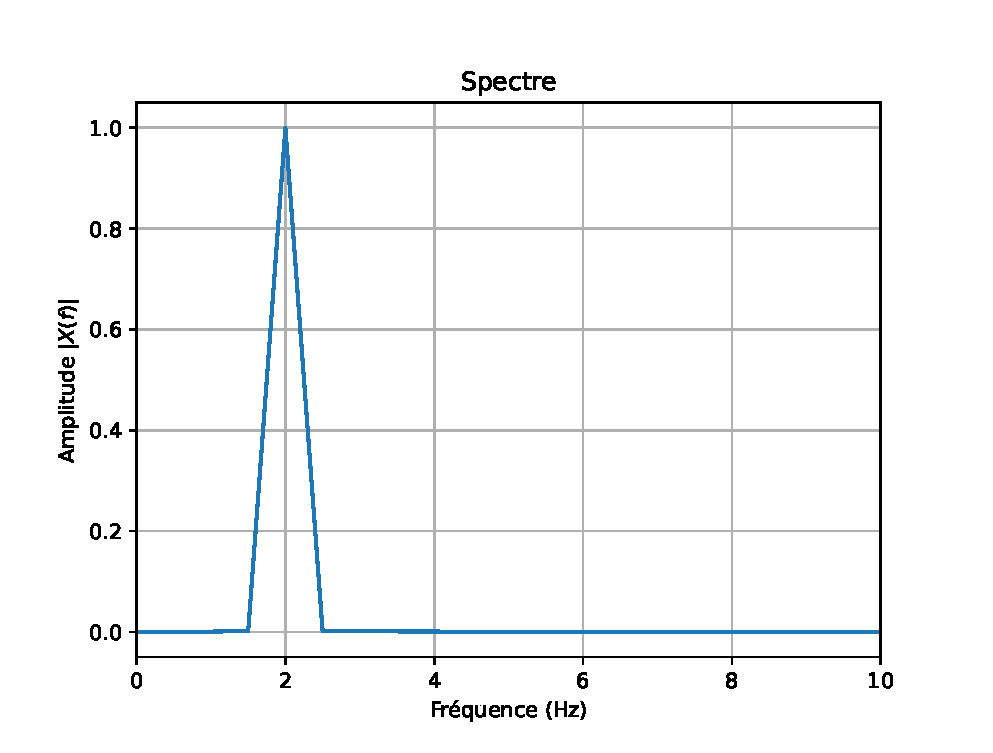
\includegraphics[scale=0.5]{sinus_4pi_spectre.eps} 

\end{minipage}
À gauche, la représentation graphique de la fonction $s$ définie pour $t>0$ par $s(t)=\sin(4\pi t)$ dont la pulsation est $\omega = 4\pi$. La fréquence $f$ est telle $\omega = 2\times \pi\times \omega $ soit $f=2$. Le spectre à droite du signal, montre l'existence unique d'une raie à $2Hz$.\\
Cette \og décomposition \fg{} est linéaire: le spectre de la somme de deux sinusoïdes est obtenu par la superposition des raies de chaque spectre.\\
\begin{minipage}{0.5\linewidth}
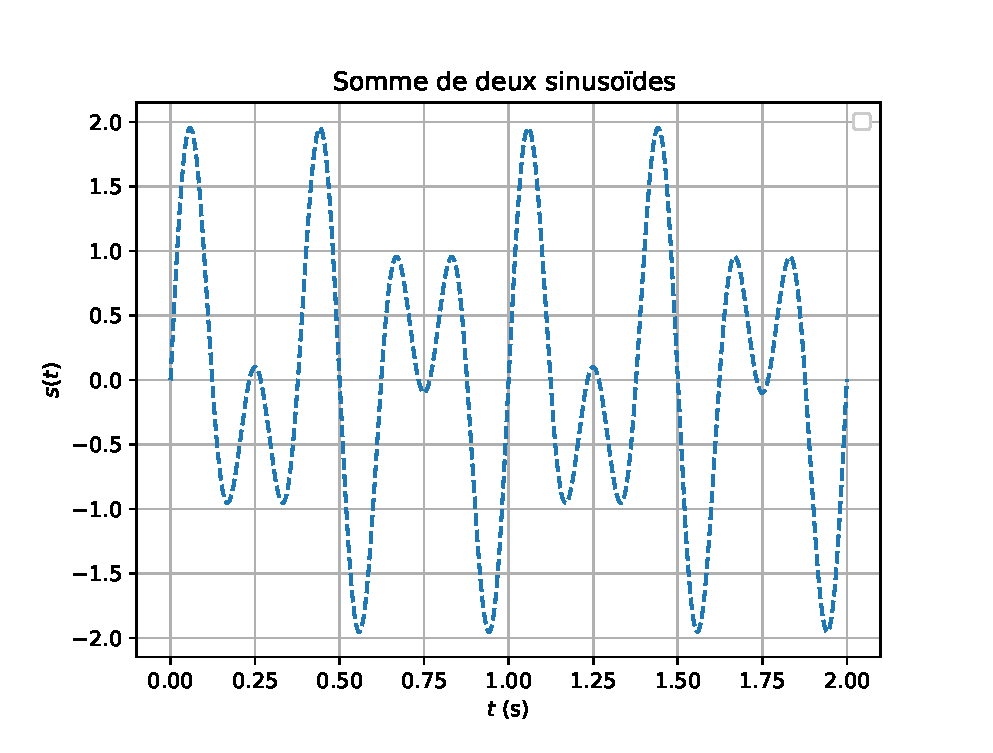
\includegraphics[scale=0.5]{somme_sin.eps} 

\end{minipage}\hfill
\begin{minipage}{0.5\linewidth}
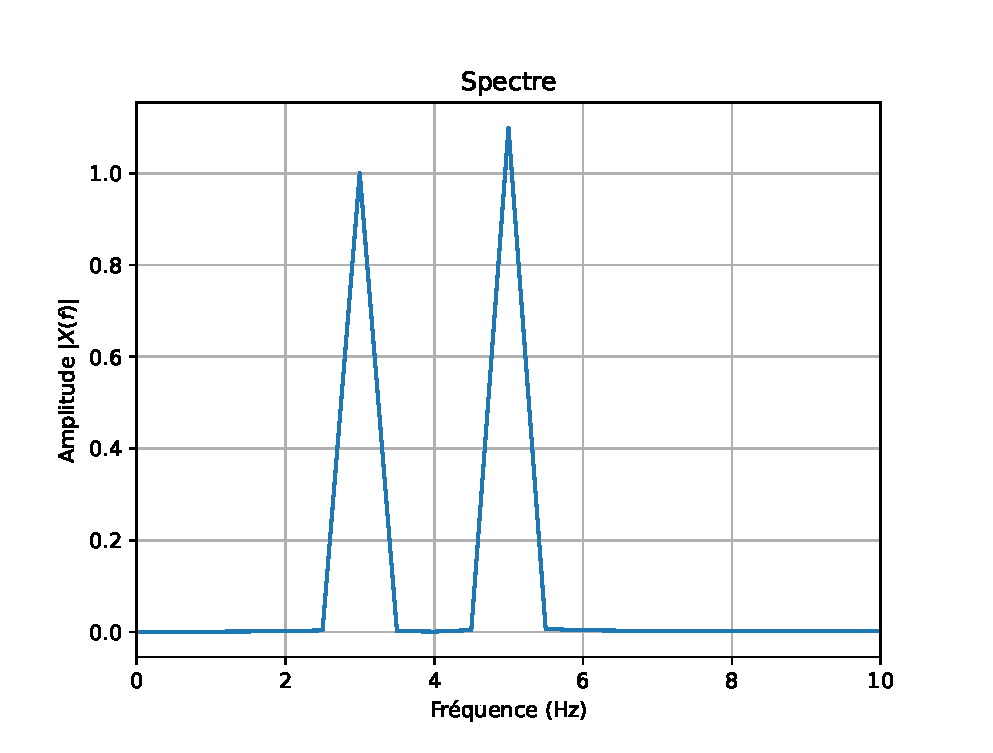
\includegraphics[scale=0.5]{somme_sin_spectre.eps} 
\end{minipage}
Le signal $s(t)=\sin(6\pi t)+ 1.1\sin(10\pi t)$ et son spectre, superposition des spectres de $s_1(t)=\sin(6\pi t)$ et $s_2(t)=\sin(10\pi t)$.\\
Joseph FOURIER est un mathématicien et physicien français né le 21 mars 1768 à Auxerre et mort le 16 mai 1830 à Paris. Il démontra non sans mal que tout signal déterministe pouvaient se décomposer en sommes de fonctions sinusoïdales\footnote{C'est le principe de sa théorie...}.\\
L'élaboration du spectre devient alors possible et directe: on peut connaître la composition spectrale de n'importe quel signal... ou presque. En fait, les calculs(que nous ne montrerons pas ici...) sont simples dans le cas d'un signal périodique mais plus complexes dans les autres cas.
Plus précisément, pour tout signal $s$ périodique de période $T$, il existe des coefficients $a_0,a_1,a_2,...$ et $b_0,b_1,b_2,...$ tels que:\\
\begin{center}
$s(t)=a_0+a_1\cos(\omega t)+b_1\sin(\omega t)+a_2\cos(2\omega t)+b_2\sin(2\omega t)+a_3\cos(3\omega t)+b_3\sin(3\omega t)+ ...$
\end{center}
où les coefficients $(a_n)$ et $(b_n)$ dépendent du seul signal $s$ et définissent les amplitudes de chaque raies et $\omega=\dfrac{2\pi}{T}$. Par exemple, considérons la fonction $s$ définie sur $\mathbb{R}$, de période $2\pi$,
telle que: 
\[
s(t)=t\ \ \mbox{ si } t\in[-\pi;\pi[
\]
On démontre que les coefficients de Fourier $a_n$ et $b_n$ de cette fonction sont tels que:
\begin{center}
$a_n=0$ et  $b_n=\dfrac{2}{n}(-1)^{n+1}$ pour tout entier $n$. \\
\begin{minipage}{0.5\linewidth}
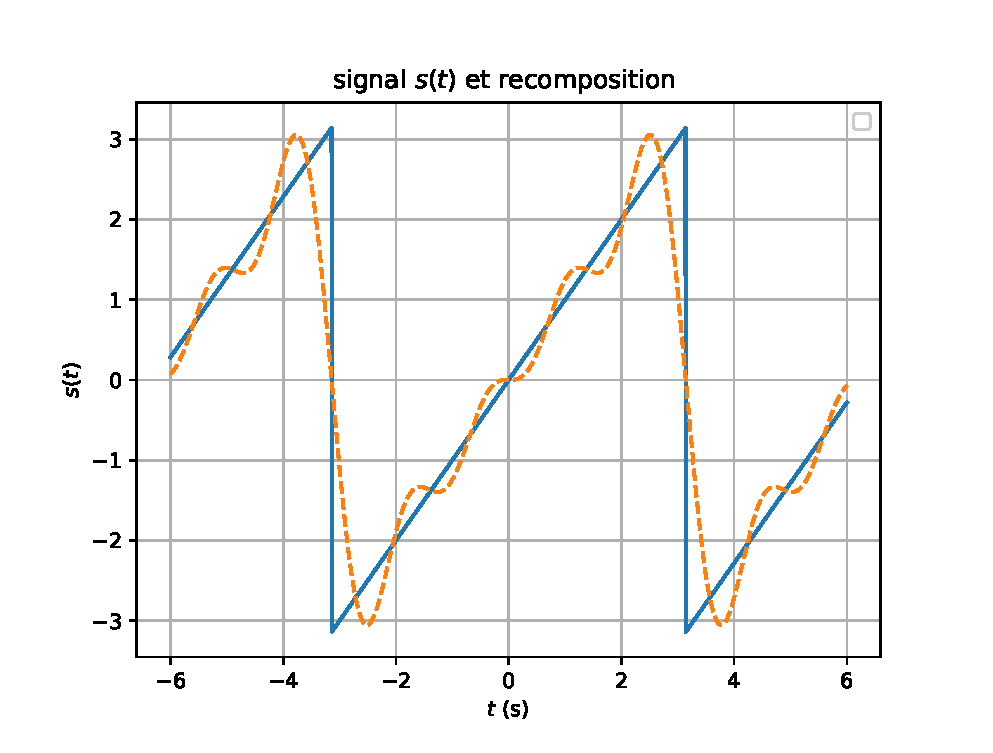
\includegraphics[scale=0.75]{exempleseriefourier.eps} 

\end{minipage}
\end{center}


 

\section{Numérisation des signaux analogiques}
Rappelons la chaîne de numérisation d'un signal analogique:\\
\begin{itemize}[label = \ding{235}]
\item \textbf{l'échantillonnage}, opération qui consiste à prélever à des intervalles de temps réguliers (ou pas...), la valeur du signal. C'est la \textbf{période} d'échantillonnage, notée $T_e$ qui détermine les temps de prélèvement.
\item \textbf{la quantification}, qui permet de projeter la valeur prélevée sur une des valeurs quantifiées. Elle est définie par le nombre $N$ de bits choisi pour représenter le signal. Rappelons:\\
\begin{center}
% \usepackage{array} is required
\begin{tabular}{|>{\centering\arraybackslash}p{3cm}|>{\centering\arraybackslash}p{2cm}|>{\centering\arraybackslash}p{2cm}|>{\centering\arraybackslash}p{2cm}|>{\centering\arraybackslash}p{2cm}|>{\centering\arraybackslash}p{2cm}|}
\hline 
Nombre de bits $N$ & 3 & 4  & 8 & 10 & 16 \\ 
\hline 
Informations possibles & &&&& \\ 
\hline 
\end{tabular} 
\end{center} 

\end{itemize}
Certainement faudra t-il avant ces deux étapes, \og passer \fg{} le signal dans un filtre passe bas! Savez vous pour quelles raisons?\par
\vspace{4cm} 

Imaginons maintenant quantifier sur 3 bits un signal échantillonné dont les valeurs extrêmes varient de $-5$ à $5$. Une certaine logique consiste à associer à :\\
\begin{itemize}[label = \ding{234}]
\item la valeur la plus basse($-5$), le nombre binaire $000$;
\item la valeur la plus haute($5$), le nombre binaire $111$

\end{itemize}
\begin{center}
\textbf{Mais quelles valeurs associer aux autres nombres binaires possibles?}
% \usepackage{array} is required
\begin{tabular}{|>{\centering\arraybackslash}p{3cm}|>{\centering\arraybackslash}p{1cm}|>{\centering\arraybackslash}p{1cm}|>{\centering\arraybackslash}p{1cm}|>{\centering\arraybackslash}p{1cm}|>{\centering\arraybackslash}p{1cm}|>{\centering\arraybackslash}p{1cm}|>{\centering\arraybackslash}p{1cm}|>{\centering\arraybackslash}p{1cm}|}
\hline 
représentation binaire & 000 & 001 & 010 & 011 & 100 & 101 & 110 & 111 \\ 
\hline 
Valeur & -5 & &&&&& & 5 \\ 
\hline 
\end{tabular} 
\end{center}



\newpage

Autres exemples et choix possibles ...\\
\includegraphics[scale=1]{sin40x3bits.eps} \\
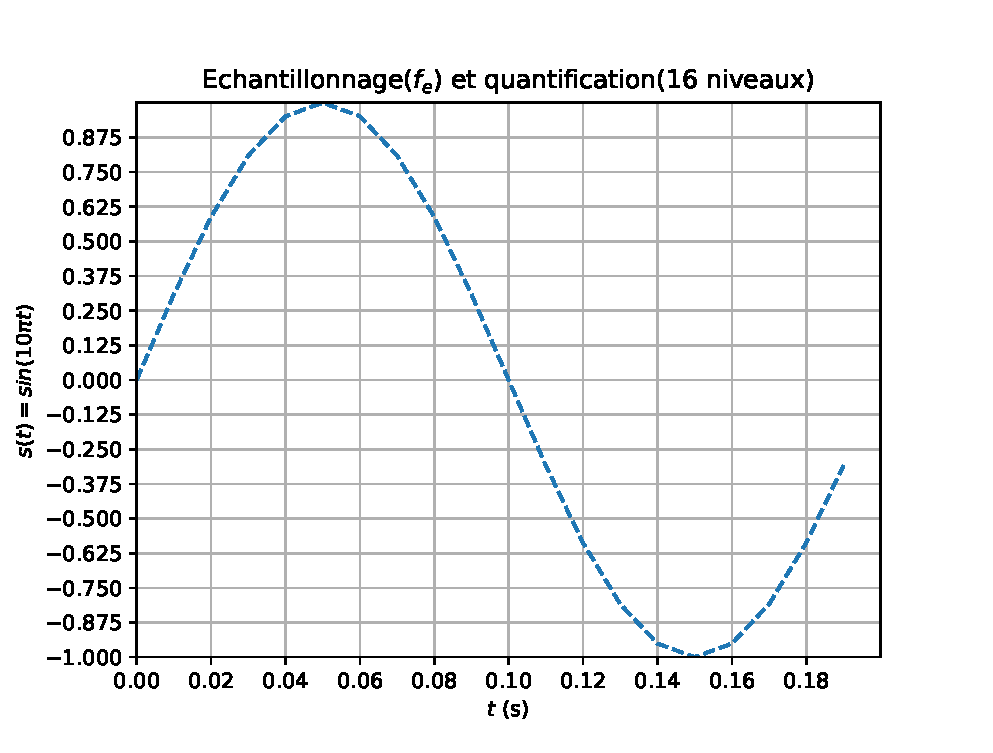
\includegraphics[scale=1]{sin50x4bits.eps} 
\newpage
\section{Spectre des signaux}
\subsection{Signal sinusoïdal}
\defprop{Le spectre d'un signal sinusoïdal de la forme:\\
 \begin{center}$s(t)=A\sin(\omega t + \phi)$ \end{center}
est composé d'une seule raie à la fréquence $f=\dfrac{\omega}{2\pi}$ d'amplitude $A$.}
La linéarisation du processus qui permet d'établir les spectres d'un signal, évoquée ci-dessus, rend aussi facile la construction des spectres des sommes de sinusoïdes...\\
Quant à leur produit il sera évoqué en exercice!
\subsection{Signal périodique quelconque}
\defprop{Le spectre d'un signal périodique quelconque de période $T$, est constitué de raies aux fréquences multiples de la fondamentale. }
Par exemple, pour un signal créneau périodique
\begin{center}
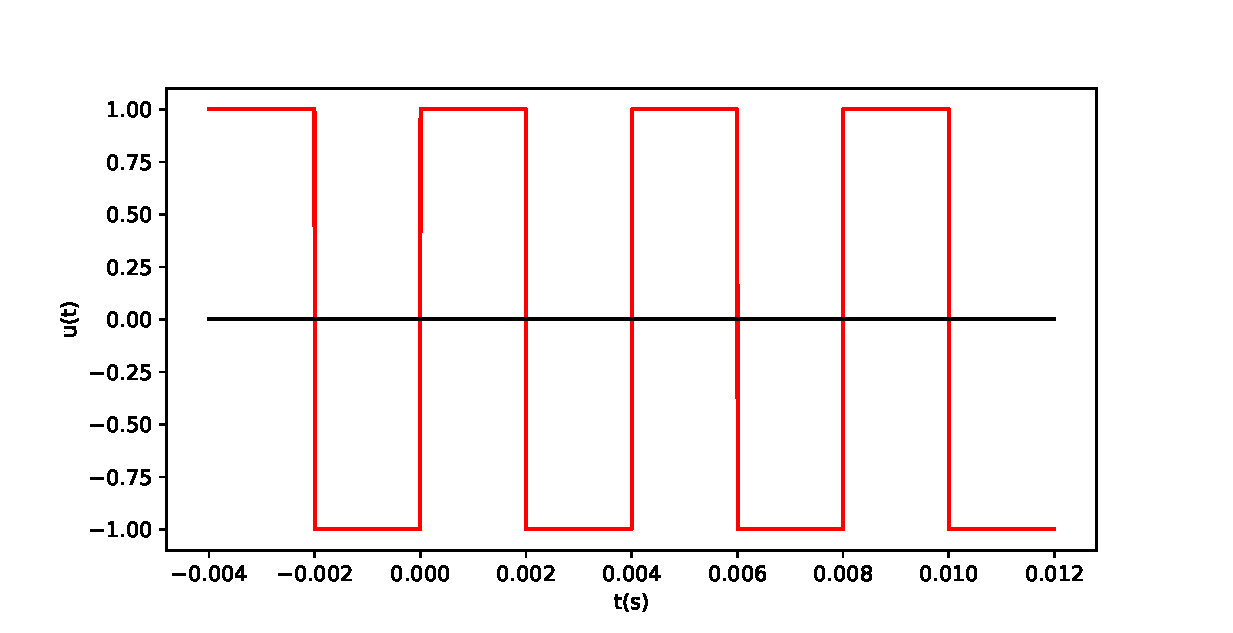
\includegraphics[scale=0.5]{signal_creneau.eps} 
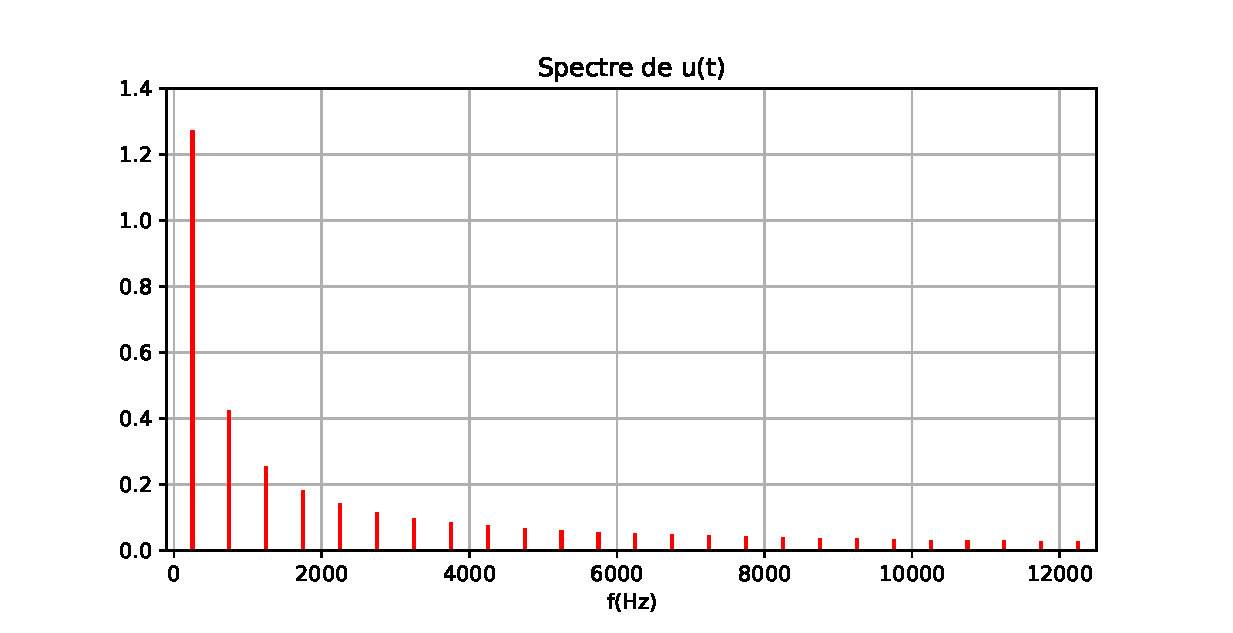
\includegraphics[scale=0.5]{spectre_creneau.eps} 
\end{center}
La décomposition de tout signal périodique en série de Fourier explique en partie ce résultat.
\newpage
\subsection{Signal quelconque non périodique}
Le spectre d'un signal quelconque, est \textbf{continue}: il n'est plus seulement constitué de raies à des valeurs précises de fréquences mais contient une plage entière de fréquence entre sa valeur minimale et maximale.\par
\vspace{4cm}
Mais, comment observer la présence de hautes fréquences, de basse fréquences dans un signal temporel?
\vspace{3cm}
\section{Effet de la numérisation sur les spectres}
La numérisation est une opération destructrice au sens où elle détériore les signaux qu'elle  représente(la compression est aussi pas mal dans le genre). Qu'en est il des spectres des signaux?\\
Quand j'échantillonne un signal, est-ce que je conserve son contenu fréquentiel?
\defprop{L'échantillonnage crée une périodisation du spectre autour de la fréquence d'échantillonnage $f_e$.}
Ce qui justifie en partie la règle de Shannon, pour éviter tout repliement de spectre!
%\section{La transformée en $z$}
\end{document}